
% Template for Elsevier CRC journal article
% version 1.2 dated 09 May 2011

% This file (c) 2009-2011 Elsevier Ltd.  Modifications may be freely made,
% provided the edited file is saved under a different name

% This file contains modifications for Procedia Computer Science

% Changes since version 1.1
% - added "procedia" option compliant with ecrc.sty version 1.2a
%   (makes the layout approximately the same as the Word CRC template)
% - added example for generating copyright line in abstract

%-----------------------------------------------------------------------------------

%% This template uses the elsarticle.cls document class and the extension package ecrc.sty
%% For full documentation on usage of elsarticle.cls, consult the documentation "elsdoc.pdf"
%% Further resources available at http://www.elsevier.com/latex

%-----------------------------------------------------------------------------------

%%%%%%%%%%%%%%%%%%%%%%%%%%%%%%%%%%%%%%%%%%%%%%%%%%%%%%%%%%%%%%
%%%%%%%%%%%%%%%%%%%%%%%%%%%%%%%%%%%%%%%%%%%%%%%%%%%%%%%%%%%%%%
%%                                                          %%
%% Important note on usage                                  %%
%% -----------------------                                  %%
%% This file should normally be compiled with PDFLaTeX      %%
%% Using standard LaTeX should work but may produce clashes %%
%%                                                          %%
%%%%%%%%%%%%%%%%%%%%%%%%%%%%%%%%%%%%%%%%%%%%%%%%%%%%%%%%%%%%%%
%%%%%%%%%%%%%%%%%%%%%%%%%%%%%%%%%%%%%%%%%%%%%%%%%%%%%%%%%%%%%%

%% The '3p' and 'times' class options of elsarticle are used for Elsevier CRC
%% The 'procedia' option causes ecrc to approximate to the Word template
\documentclass[3p,times,procedia]{elsarticle}

%% The `ecrc' package must be called to make the CRC functionality available
\usepackage{ecrc}
\usepackage{hyperref}
\usepackage{amsmath}

%% The ecrc package defines commands needed for running heads and logos.
%% For running heads, you can set the journal name, the volume, the starting page and the authors

%% set the volume if you know. Otherwise `00'
\volume{00}

%% set the starting page if not 1
\firstpage{1}

%% Give the name of the journal
\journalname{Procedia Computer Science}

%% Give the author list to appear in the running head
%% Example \runauth{C.V. Radhakrishnan et al.}
\runauth{Ying Liu, Chao Xiang}

%% The choice of journal logo is determined by the \jid and \jnltitlelogo commands.
%% A user-supplied logo with the name <\jid>logo.pdf will be inserted if present.
%% e.g. if \jid{yspmi} the system will look for a file yspmilogo.pdf
%% Otherwise the content of \jnltitlelogo will be set between horizontal lines as a default logo

%% Give the abbreviation of the Journal.
\jid{procs}

%% Give a short journal name for the dummy logo (if needed)
\jnltitlelogo{Procedia Computer Science}

%% Provide the copyright line to appear in the abstract
%% Usage:
%   \CopyrightLine[<text-before-year>]{<year>}{<restt-of-the-copyright-text>}
%   \CopyrightLine[Crown copyright]{2011}{Published by Elsevier Ltd.}
%   \CopyrightLine{2011}{Elsevier Ltd. All rights reserved}
\CopyrightLine{2016}{The Authors. Published by Elsevier B.V.\newline Selection and/or peer-review under responsibility of ITQM2016}


%% Hereafter the template follows `elsarticle'.
%% For more details see the existing template files elsarticle-template-harv.tex and elsarticle-template-num.tex.

%% Elsevier CRC generally uses a numbered reference style
%% For this, the conventions of elsarticle-template-num.tex should be followed (included below)
%% If using BibTeX, use the style file elsarticle-num.bst

%% End of ecrc-specific commands
%%%%%%%%%%%%%%%%%%%%%%%%%%%%%%%%%%%%%%%%%%%%%%%%%%%%%%%%%%%%%%%%%%%%%%%%%%

%% The amssymb package provides various useful mathematical symbols
\usepackage{amssymb}
%% The amsthm package provides extended theorem environments
%% \usepackage{amsthm}

%% The lineno packages adds line numbers. Start line numbering with
%% \begin{linenumbers}, end it with \end{linenumbers}. Or switch it on
%% for the whole article with \linenumbers after \end{frontmatter}.
%% \usepackage{lineno}

%% natbib.sty is loaded by default. However, natbib options can be
%% provided with \biboptions{...} command. Following options are
%% valid:

%%   round  -  round parentheses are used (default)
%%   square -  square brackets are used   [option]
%%   curly  -  curly braces are used      {option}
%%   angle  -  angle brackets are used    <option>
%%   semicolon  -  multiple citations separated by semi-colon
%%   colon  - same as semicolon, an earlier confusion
%%   comma  -  separated by comma
%%   numbers-  selects numerical citations
%%   super  -  numerical citations as superscripts
%%   sort   -  sorts multiple citations according to order in ref. list
%%   sort&compress   -  like sort, but also compresses numerical citations
%%   compress - compresses without sorting
%%
%% \biboptions{comma,round}

% \biboptions{}

% if you have landscape tables
\usepackage[figuresright]{rotating}

% put your own definitions here:
%   \newcommand{\cZ}{\cal{Z}}
%   \newtheorem{def}{Definition}[section]
%   ...

% add words to TeX's hyphenation exception list
%\hyphenation{author another created financial paper re-commend-ed Post-Script}

% declarations for front matter

\begin{document}

\begin{frontmatter}

%% Title, authors and addresses

%% use the tnoteref command within \title for footnotes;
%% use the tnotetext command for the associated footnote;
%% use the fnref command within \author or \address for footnotes;
%% use the fntext command for the associated footnote;
%% use the corref command within \author for corresponding author footnotes;
%% use the cortext command for the associated footnote;
%% use the ead command for the email address,
%% and the form \ead[url] for the home page:
%%
%% \title{Title\tnoteref{label1}}
%% \tnotetext[label1]{}
%% \author{Name\corref{cor1}\fnref{label2}}
%% \ead{email address}
%% \ead[url]{home page}
%% \fntext[label2]{}
%% \cortext[cor1]{}
%% \address{Address\fnref{label3}}
%% \fntext[label3]{}

\dochead{Information Technology and Quantitative Management (ITQM 2016)}
%% Use \dochead if there is an article header, e.g. \dochead{Short communication}
%% \dochead can also be used to include a conference title, if directed by the editors
%% e.g. \dochead{17th International Conference on Dynamical Processes in Excited States of Solids}

\title{Hybrid learning net: a novel architecture for fast learning}

%% use optional labels to link authors explicitly to addresses:
%% \author[label1,label2]{<author name>}
%% \address[label1]{<address>}
%% \address[label2]{<address>}

\author[a]{Ying Liu}
\author[a]{Chao Xiang}

\address[a]{University of Chinese Academy of Sciences, Beijing 100049, China}

\begin{abstract}
%% Text of abstract
Currently, neural networks have 
succeeded in object recognition 
tasks based on images, natural 
language translation, and voice 
recognition, to name a few. 
However, neural nets are customly 
built for different applications 
and vary a lot in achitectures 
and model hyperparameters like 
learning rate and parameter 
initialization, what's worse,
these hyperparameter settings 
generally play a big role in 
performances of training and 
testing, and the best settings 
for specific applications are so 
far only available by manually 
repeatly trying different 
configurations which is really 
huge work. We, thereby, present 
a novel neural network achitecture,
called Hybrid Learning Net($\mathbf{HLN}$), 
with Self Organizing Maps(SOMs) 
embedded in each layer to learn 
from samples in $\mathbf{both}$ 
unsupervised and supervised way, 
targeting to achieve a much
$\mathbf{faster}$ net learning for general 
applications with good robustness
to a few key hyperparameters such 
as the parameter initialization
and the net strcuture variation. 
We've also experimented our 
architecture over the MNIST 
dataset, it has proved the 
impressive improvement on both 
training and testing phases
of general applications, 
say compared to the traditional
architecture, our method speed up
the training process by up to 
$\mathbf{40}$ times, which only
take $\mathbf{1}$ epoch to get 
an testing accuracy of over
$\mathbf{87.5\%}$, and takes
no more than $\mathbf{3}$ epoches
to reach a profound accuracy of 
over $\mathbf{91.3\%}$.
In addition, on big scale
of input dimension and/or with deeper 
architecture, where the traditional
architecture fails to learn at all,
our method still have a fast learning,
and can retrieve the same testing 
accuracy on MNIST.
Moreover, we have discovered 
some interesting facts about 
neural network trainings, 
such as neuron activation 
sparsity is strongly 
correlated to the training loss 
within certain cases which may shed 
a little light on how such 
architecture really works.
\end{abstract}

\begin{keyword}
hybrid learning; neural network; general application; sparsity; SOM; MNIST; fast learning

%% keywords here, in the form: keyword \sep keyword

%% PACS codes here, in the form: \PACS code \sep code

%% MSC codes here, in the form: \MSC code \sep code
%% or \MSC[2008] code \sep code (2000 is the default)

\end{keyword}

\end{frontmatter}

\correspondingauthor[*]{Corresponding author. Tel.: +86-183-0114-2368;}
\email{xiangchao215@mails.ucas.ac.cn}

%%
%% Start line numbering here if you want
%%
% \linenumbers

%% main text
\section{Introduction}
\label{main}
Since the first mathematical model 
of artificial neural network was 
proposed in 1943\cite{mcculloch1943logical}, 
the neural network has been 
designed into many architectures, 
such as Convolutional Neural 
Networks(CNNs) for image 
recognition
\cite{krizhevsky2012imagenet}, 
Recurrent Convolutional Neural 
Networks(R-CNNs) for object 
detection in 
videos\cite{girshick2015fast}, 
and Long Short Term Memorys(LSTMs)
for speech recognition
\cite{graves2013hybrid} and many, 
many more to make it a list. 
These specially designed neural 
network models are trained by 
lots of efficient methods with 
tons of carefully chosen little 
skills which we may call tricks. 
Such neural network architectures
suit well for their specific 
applications but may have plain 
or worse performances on others, 
and their best performances 
rely heavily on hyperparameter 
configuration in general. Thus, 
it is an in-demand job to propose 
a relatively universal 
architecutre that enables equal 
or similar performances among 
varied applications.

We notice that, although there're 
plenty of choices to train a 
neural network, literally all 
these methods can be reduced into
3 categories, supervised learning
\cite{lecun1990handwritten}, 
unsupervised learning
\cite{vincent2010stacked}, 
and the semi-supervised
\cite{chapelle2009semi}.
In supervised learning, 
one can only train a model from 
labeled samples, however in real 
applications, labeling a large 
dataset is a tough and costly 
task, the unlabeled ones are 
therefore the primary data 
available. To make use of the 
majority unlabeled data, a few 
unsupervised training algorithms 
arose. These unsupervised learning
methods, denoted as pretraining, 
attempt to produce an optimized 
parameter initialization
\cite{le2013building}.
Thus such unsupervised techniques 
can only be applied before the 
supervised training phase, once 
the supervised begins, the 
unsupversied learning will become 
unavailable for the model.
While the semi-supervised learning
allows the model to learn from
both labeled and unlabeled samples 
at the same time, however they use a
regularizer to embed the semi-supervised
learner to original optimizing object,
and generally a balance constraint is
required to avoid the trival solution
\cite{socher2011semi}.
Such a enhanced learner brings more 
hyperparameters(say the balance 
constraint), making it even more 
difficult to search for best settings
for current architectures. 
Additionally, this integration way 
makes it impossible to separate the 
two learners as the semi-supervised 
regularizer is built on the supervised 
learner, and therefore requires an 
early supervised training alone with 
profound labeled data before the 
semi-supervised regularizer can be
applied.
Thus we introduce a new architecture
that learn in both supervised and 
unsupervised ways at the same time,
and requires no extra techniques on
training. Our architecture, Hybrid
Learning Nets(HLNs), made of 
stacked layers, with each hidden
layer embedded with a Self Organizing
Map(SOM), training in
the simplest way of backprop, 
demonstrate much faster learning
capability and remain robust to 
parameter initialization and
network configuration such as the net
depth of layer.

%\subsection{Our contributes}
The main contributions of our work are:
\begin{itemize}
\item We propose HLN, a SOM-embedded 
architecture to learn both unlabeled 
and labeled data at the same time.
\item Our architecture HLN overcomes
the problem brought by traditional 
semi-supervised learning methods that 
the semi-supervised learning requires
an early standalone training for the
supervised learner which contradicts
with the key condition: no enough 
labeled data is provided.
\item The HLN uses a SOM embedding 
coupling the first hidden layer near 
to the input layer, to learn a cluster 
mapping function from the cheap and 
massive unlabeled data, and this process
can occur at any time, no matter the 
supervised learning begins or not,
they're completely separated.
For deeper hidden layers, each of them 
also has a SOM-embedding coupled, 
but can only learn from labeled data.
\item The experimental result shows HLNs
speed up the whole training a lot.
\item Our architecture demonstrates a 
good robustness to some hyperparameters
which may slightly relax the work of 
manually searching for best settings
of hyperparameters by repeatly trying
different configurations and run the
whole training and testing over and 
over again.
\end{itemize}
HLN is implemented in Python and all
our code and results of experiments
in detail are available at
\url{https://github.com/hiroki-kyoto/hybrid-learning-net}.

%\subsection{The organization of this artical}
The rest of the article is as follows.
In section 2 we describe existing
semi-supervised algorithms for neural
network models, recall
the SOM and explore a different
training method for SOM when applied in
the neural network embedding.
In section 3, we introduce our novel
architecture HLN, show how to
embed SOMs into deep architectures of
neural nets.
In section 4 we explain the exact 
training theory for HLNs.
Section 5 gives experimental
comparisons between nets with HLN
architecture and without, and the
last section concludes.

\section{Related work and backgrounds}

\subsection{Semi-supervised learning for
neural network}
A key assumption in semi-supervised 
algorithms developed so far, is the 
structure assumption: two samples with 
similar distribution on the same mapping 
structure tend to have high probability 
of belonging to the same class. Based on 
this assumption, one can use large 
unlabeled data to uncover such 
structures. There're already a few 
algorithms dedicated to do this,
such as cluster kernels
\cite{chapelle2003cluster},
Low Density Separation(LDS)
\cite{chapelle2005semi},
label propagation
\cite{zhu2002learning},
to name a few.
In such algorithms, designing a regularizer
to enable the model to learn the representation
or structure of raw data, in order to improve
the supervised learning performance, becomes
the key point.

Let's firstly focus on the general algorithm
description of semi-supervised learning.
Given a set of unlabeled samples,
$\mathbf{X}=\{\mathbf{x}_1,\cdots,
\mathbf{x}_N\}(\mathbf{x}\in\mathbb{R}^d)$,
and the similarity labels between any
$\mathbf{x}_i$ and $\mathbf{x}_j$,
$\mathbf{W}=\{W_{ij}|i,j=1,\cdots,N\}$,
we're to find the best embedding function, 
$f(\mathbf{x})$, for each sample $\mathbf{x}_i$, 
to minimize:
\begin{equation}
\Delta_{f}=
	\sum^{N}_{i=1}
	\sum^{N}_{j=1}
	L\left(
	f(\mathbf{x}_i),
	f(\mathbf{x}_j),
	W_{ij}
	\right)
\label{eq:1}
\end{equation}
To explain it,
\begin{itemize}[]
\item $L(\cdot)$ is the loss function of 3 
variables: 
$\left<
		f(\mathbf{x}_i),
		f(\mathbf{x}_j),
		W_{ij}
		\right>$, 
such as 
		$$L\left(
		f(\mathbf{x}_i),
		f(\mathbf{x}_j),
		W_{ij}
		\right) = 
		\max\left(
		0,
		\|f(\mathbf{x}_i)-
		f(\mathbf{x}_j)
		\|-W_{ij}
		\right)$$
\item $f(\mathbf{x})\in\mathbb{R}^n$ is the 
embedding function, it tries to produce a 
vector from $\mathbf{x}_i$, similar to that 
of $\mathbf{x}_j$ with $W_{ij}=0$,
and disimilar with $W_{ij}=1$.
\item $W_{ij}\in \mathbb{R}$ is the similarity 
label of the sample pair
$\left<
		\mathbf{x}_i,
		\mathbf{x}_j
		\right>$ from $\mathbf{X}$.
\end{itemize}

\emph{Label Propagation(LP)}
\cite{zhu2002learning} 
is one of the most efficient algorithms using 
the semi-supervised learning scheme as 
described above in equation~\ref{eq:1}. 
It adds a Laplacian Eigenmap type 
regularization to a nearest neighbor 
classifier:
\begin{equation}
	\min_f
	\sum^L_{i=1}
	\left\|
	\vec{f}_i-\mathbf{\hat{y}}_i
	\right\|^2 +
	\lambda
	\sum^{L+U}_{i=1}
	\sum^{L+U}_{j=1}
	W_{ij}
	\left\|
	\vec{f}_i-\vec{f}_j
	\right\|^2
	\label{eq:2}
\end{equation}
$L$ is a labeled sample set of $\mathbf{X}$, 
and $U$ is 
a unlabeled one, the right part of 
equation~\ref{eq:2} is the semi-supervised 
regularizer,
the left part is for supervised learning only.
Parameter $\lambda$ is the balance constraint. 
LP trains the classifier $f(\cdot)$ to give
two examples with high similarity $W_{ij}$
the same label, and the neighbors of neighbors
tend to get the same label by transitivity.
The two points make its name \emph{label
propagation}.

For neural network model,
we replace $f(\cdot)$ with equation as follow,
\begin{equation}
	y_i=\sum_j w_j^{M+1,i}y^M_j(\mathbf{x})
	+b^{M+1,i},\quad i=1,\cdots,D
\label{eq:3}
\end{equation}
and such that
\begin{equation}
	f(\mathbf{x}) = \vec{y}=
	\left(y_1,y_2,\cdots,y_D\right)
\label{eq:4}
\end{equation}
The equation~\ref{eq:3} describe the simplest 
neural model with $M$ hidden layers, $D$ is 
the output dimension, $f_i(\mathbf{x})$ 
computes the output of $i^{th}$ neuron in the
$(M+1)^{th}$(index starts from 0) 
layer(the output layer of the net model) 
and $y^{M}_j$ is the $j^{th}$ hidden
neuron on $M^{th}$ layer, $w^{M+1,i}_j$
is the connection weight from $j^{th}$
neuron in $M^{th}$ layer to 
$i^{th}$ neuron in output layer.
$b^{M+1,i}$ is the bias for the $i^{th}$
neuron in $(M+1)^{th}$ layer.
To get $y_j^M$, just follow the equation as
\begin{equation}
	y^k_i(\mathbf{x}) = \sigma\left(
		\sum_j w_j^{k,i}y_j^{k-1}
		+b^{k,i}
	\right),k>1
	\label{eq:5}
\end{equation}
and when it comes to the first hidden layer,
\begin{equation}
	y^1_i(\mathbf{x})=
	\sigma\left(\sum_jw_j^{1,i}x_j
	+b^{1,i}\right)
	\label{eq:6}
\end{equation}
$\sigma$ can be any non-linear function, such as
the sigmoid $\left(1+e^{-x}\right)^{-1}$, 
$tanh(x)=\frac{e^x-e^{-x}}{e^x+e^{-x}}$ and 
the latest ReLU $\sigma(x)=\max(0,x)$ and a few
more. Notice that a nonlinear activation
function is often required when the neural
network model is used in a classification
application.

\subsection{Traditional way for 
semi-supervised embedding}
As described in last subsection, 
the traditional way to embed semi-supervised 
learning ability into a neural net is through 
a weighted regularizer, which is practically 
adding a semi-supervised loss $\Delta_f$
onto the supervised learning loss
\cite{weston2012deep}, thus the learning 
problem turns to be minimizing:
\begin{equation}
	\sum^L_{i=1}\ell\left(
	f(\mathbf{x}_i),\mathbf{\hat{y}}_i
	\right) +
	\lambda\sum^{L+U}_{i=1}\sum^{L+U}_{j=1}
	L\left(
	f(\mathbf{x}_i),
	f(\mathbf{x}_j),
	W_{ij}
	\right)
	\label{eq:7}
\end{equation}
and in most efficient algorithms Euclidean 
metric is used for the loss.

\subsection{Self Organizing Map}
The Self Organizing Map(SOM) is an effective 
software tool for the visualization of 
high-dimensional data. It can also be used 
as an automatic clustering method. The SOM
consists of a two-dimensional regular grid
of nodes. The models are automatically 
organized into a meaningful two-dimensional
order in which similar models are closer to
each other in the grid than the more dissimilar
ones\cite{kohonen1998self}.
It use such rules to update models:
\begin{equation}
	\mathbf{m}_i(t+1)=\mathbf{m}_i(t)+
	h_{c(x),i}\left(
	\mathbf{x}(t)-\mathbf{m}_i(t)
	\right)
	\label{eq:8}
\end{equation}
and the learning rate is dynamically determined
as
\begin{equation}
	h_{c(x),i} = \alpha(t)\exp\left(
	-\frac{\|\mathbf{r}_i-\mathbf{r}_c\|^2}
	{2\sigma^2(t)}
	\right)
	\label{eq:9}
\end{equation}
where $\mathbf{m}_i\in\mathbb{R}^n$ 
is the $i^{th}$ model vector, 
$\mathbf{x}$ is an input pattern,
$c(x)$ relates to the best match vector index
in $\mathbf{m}$ for input pattern $\mathbf{x}$,
and $\alpha(t)$ is a learning rate that 
decreases with training preceeding.
$\mathbf{r}$ is the model vector location in 
the map, and $\sigma(t)$ corresponds to the 
width of the neighborhood function, which 
also decreases monotonically with the 
regression steps.


\section{Our architecture: 
the Hybrid Learning Net}
We propose the Hybrid Learning Net(HLN) as
an architecture to enhance arbitrary nets
on their training efficiency and robustness 
to some hyperparameters.
Each layer in the HLN architecture embeds a
SOM into its original layer, for the simplest
situation where neurons connected in fully
connected way, which we call the Fully 
Connected Neurons(FCN) architecture, we have 
such an embedding solution as described in 
figure~\ref{fig:1}.

\begin{figure}[h]
	\centerline{
		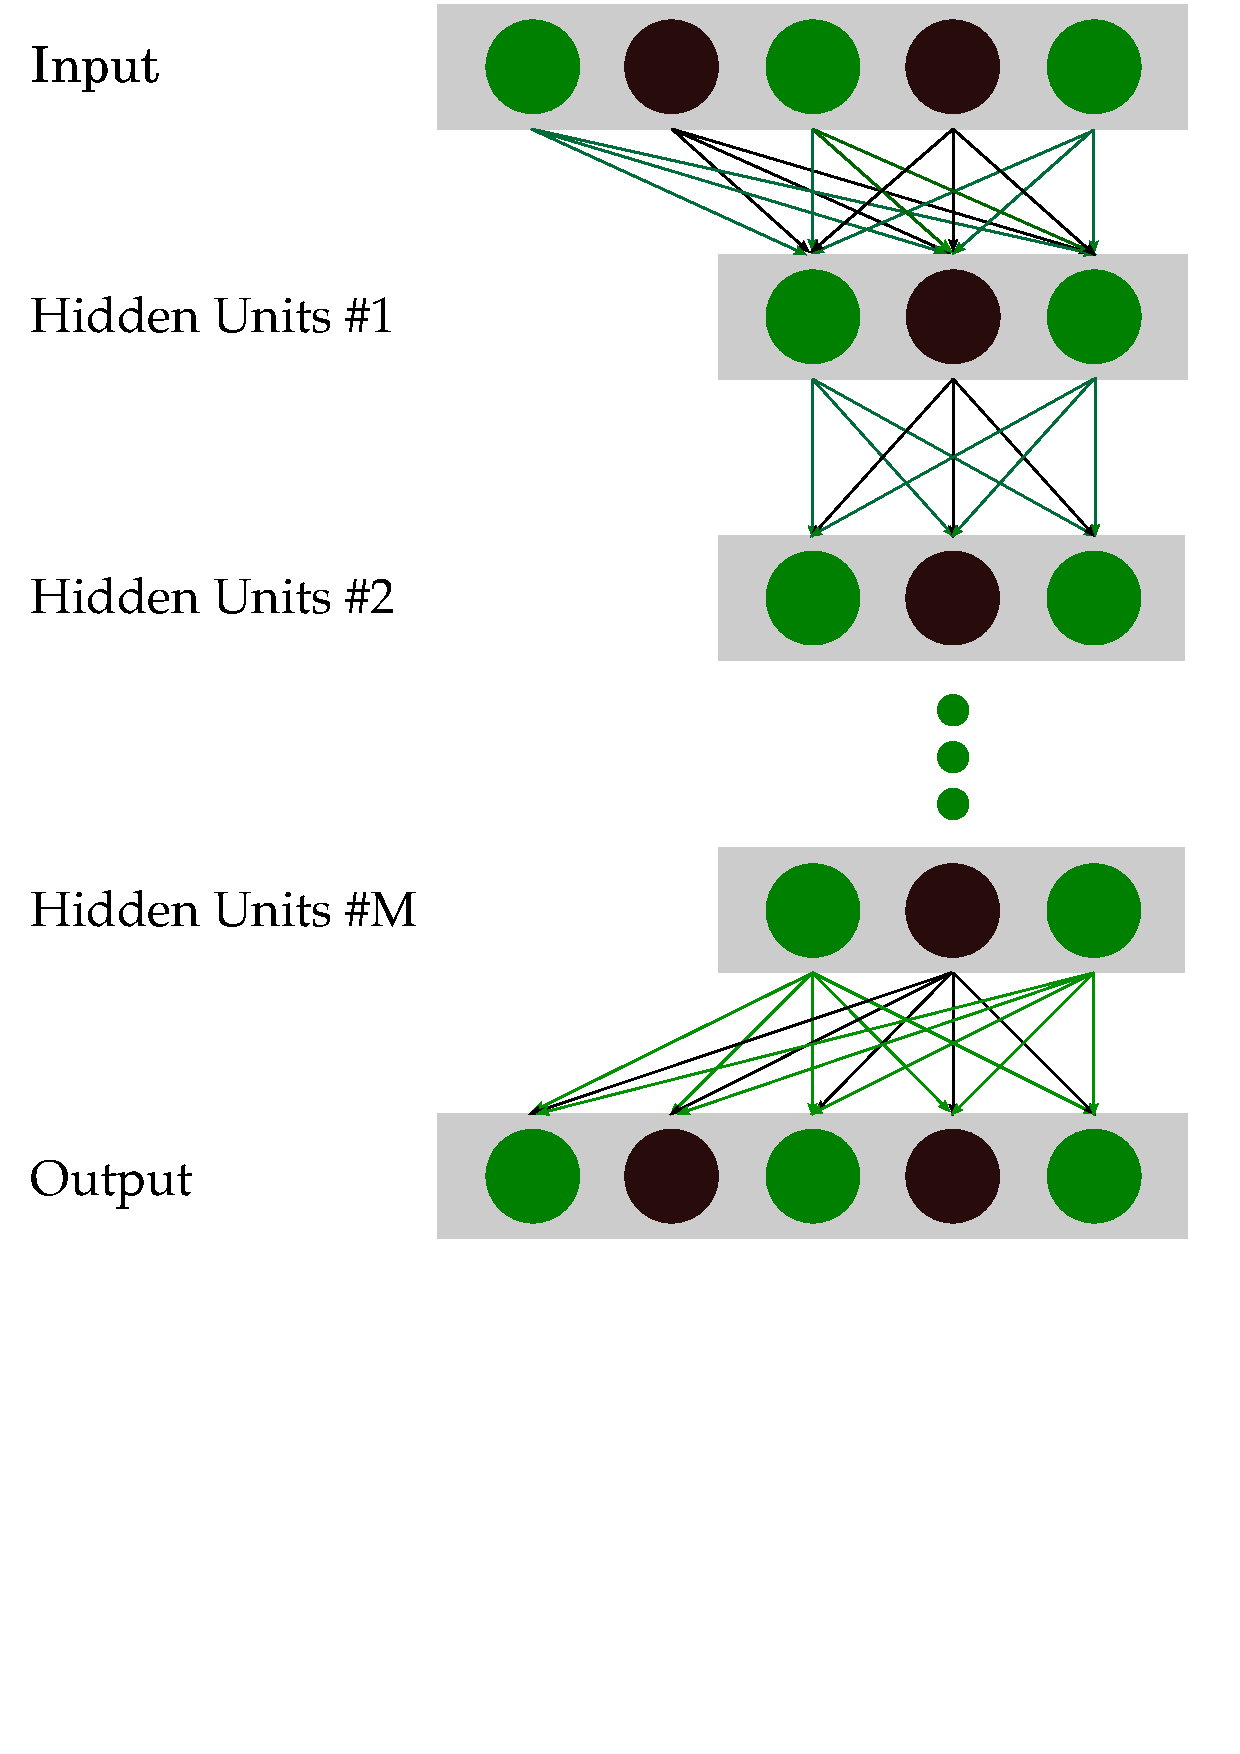
\includegraphics[width=3in]{FCN}
		\hspace*{5mm}
		\includegraphics[width=3in]{HLN}
	}
\caption{(a) FCN architecture; 
	(b) HLN architecture.}
	\label{fig:1}
\end{figure}

In the HLN architecture from figure~\ref{fig:1},
$h(x)$ is an unifying function we proposed for 
SOMs to convert from pattern disimilarity
$\|\mathbf{x}-\mathbf{m}_i\|$, into
a semi-supervised learning factor for
different hidden units. The semi-supervised
learning factors as a whole act as a 
dynamic neuron activation sparsity mask for 
each hybrid learning layer.
It works in a way like the Dropout 
technique\cite{srivastava2014dropout}, 
enabling the neural nets 
to improve the model robustness and prevent
overfitting by learning their submodels for 
each batch. However, the HLN differs from 
techniques like the Dropout in which, 
the HLN does not generate sparsity with 
randomness, she uses the SOM
to unsupervisedly learn the \emph{static}
policy of neuron-activation distribution for
each layer, the net sparsity generator thereby
will stablize with training steps, and the
randomness in sparsity will disappear 
automatically.
We propose $h(x)$ with the form as followings,
\begin{equation}
	\delta_{max} = \max_i\left(
	\|\mathbf{m}_i-\mathbf{x}\|+\epsilon
	\right)
	\label{eq:10}
\end{equation}
$\delta_{max}$ is the maximum disimilarity
between an arbitrary vector in $\mathbf{m}$
and the input pattern vector $\mathbf{x}$,
$\delta_{min}$ is similar,
\begin{equation}
	\delta_{min} = \min_i\left(
	\|\mathbf{m}_i-\mathbf{x}\|+\epsilon
	\right)
	\label{eq:11}
\end{equation}
and the scale of all disimilarities is
\begin{equation}
	\delta_{scale} = 
	\frac{\mathbf{\delta}_{min}}
	{\mathbf{\delta}_{max}-
	\mathbf{\delta}_{min} + \epsilon}
	\label{eq:12}
\end{equation}
Finally we unify the disimilarities and convert
them into sparsity mask as
\begin{equation}
	h(x)|_{x=\|\mathbf{m}_i-\mathbf{x}\|}=
	\frac{\delta_{max}\cdot\delta_{scale}}
	{\left\|\mathbf{m}_i-\mathbf{x}\right\|
	+\epsilon}-\delta_{scale}
	\label{eq:13}
\end{equation}
in which $\mathbf{m}_i$ and $\mathbf{x}$ is the
same way defined in equation~\ref{eq:8}.
$\epsilon$ is a constant of pretty small value
like $\epsilon=10^{-5}$ to avoid 
\emph{division-by-zero} errors that may, 
though not very likely occur. Notice that
if any other metrics be preferred, we can
always replace the pattern disimilarity
$\|\mathbf{m}_i-\mathbf{x}\|$ with its
corresponding form.
$f(s,o)$ is the function to combine the 
sparsity mask $s$ generated by $h(\cdot)$ 
and the fully connected linear summation 
output $o$. In most cases, we choose the
multiplication operator,
\begin{equation}
	f(s,o) = s\cdot o = 
	h\left(
	\left\|
	\mathbf{m}_i-\mathbf{y^{k-1}}
	\right\|
	\right)
	\cdot
	\sum_j
	\left(
	w_j^{k,i}y_j^{k-1}
	\right)
	+b^{k,i},k>1
	\label{eq:14}
\end{equation}
where $w$, $y$, $b$, $i$, $j$, $k$ is the
same denotion as in equation~\ref{eq:5}.
For the computing flow described in 
figure~\ref{fig:1}, $f(\cdot) $ is followed 
by an activation function, it can be any 
arbitrary nonlinear function that takes 
only one dimension inputs and outputs a 
single real, such as the sigmoid function, 
$tanh(x)$ and the ReLU. With the new 
architecture, we update the computing rules 
in equations~(\ref{eq:5}) and (\ref{eq:6}) as 
\begin{equation}
	y_i^k(\mathbf{x})=
	\sigma\left(
	h\left(
	\left\|
	\mathbf{m}_i^k-y^{k-1}(\mathbf{x})
	\right\|
	\right)\cdot
	\sum_j\left(
	w_j^{k,i}y_j^{k-1}(\mathbf{x})
	\right) + b^{k,i}
	\right), k>1
	\label{eq:15}
\end{equation}
and for the very first hybrid learning layer,  
\begin{equation}
	y_i^1(\mathbf{x})=
	\sigma\left(
	h\left(
	\left\|
	\mathbf{m}_i^1-\mathbf{x}
	\right\|
	\right)\cdot
	\left(
	\sum_j w_j^{1,i}x_j
	\right) + b^{1,i}
	\right)
	\label{eq:16}
\end{equation}
where $m^k_i$ denotes the $i^{th}$ vector
in the $k^{th}$ SOM of the net(all indexes
start from 1), $\sigma$ is a nonlinear 
activation function.
The equations~(\ref{eq:3}) and (\ref{eq:4})
require no update since the output layer
of the net is not involved in the 
architecture shifting.

\section{The training theory for HLNs}
Let's compare the embedding theories between
HLNs and the ones mentioned in the section of
\emph{Related work and backgrounds}.
The existing semi-supervised algorithms
embed a regularizer into the supervised 
learner, making it impossible to train both of
the supervised learner and the unsupervised
separately. As analyzed before, performances
of such regularizer solutions depends on the
standalone supervised pretraining for which
a profound labeled data is required.
However, in our architecture HLN, we assign
each of the learning methods a completely
separate optimizing object, with no priority
orders restricted.\\
For the supervised learning, we may have such
form of optimizing object as
\begin{equation}
	\arg \min_g \sum_{i=1}^L\ell\left(
	g(\mathbf{x}_i),
	\mathbf{\hat{y}}_i
	\right)
	\label{eq:17}
\end{equation}
where $g(\mathbf{x})$ is the function describing
the mapping from the input 
$\mathbf{x}\in\mathbb{R}^d$ to the output
$\mathbf{y}\in\mathbb{R}^n$, parameterized with
the neural connection weights $\mathbf{W}$ and 
the biases $\mathbf{b}$ for all non-input 
layer neurons in the HLN architecture.
This equation~\ref{eq:17} may become the 
following one when Enclidean metrics be 
applied for the loss,
\begin{equation}
	\arg \min_{\mathbf{W},\mathbf{b}}
	\frac{1}{2}
	\sum_{i=1}^L
	\left\|
	y^k(
	\mathbf{x}_i)\big|_{\mathbf{W},\mathbf{b}}-
	\mathbf{\hat{y}}_i
	\right\|^2
	\label{eq:18}
\end{equation}
For the unsupervised learning, the optimizing
objects are
\begin{equation}
	\arg \min_{\mathbf{m}^k}
	\sum_i^{L+U}
	\left(
	\min_j\left(
	\left\|
	\mathbf{m}^k_j-\mathbf{x}^k_i
	\right\|
	\right)
	\right),\quad k=1,2,\cdots
	\label{eq:19}
\end{equation}
with the predefined notation:
\begin{equation}
	\mathbf{x}_i^k=
	\left\{
		\begin{aligned}
			\mathbf{x}_i,\quad & k=1\\
			y^{k-1}(\mathbf{x}_i),\quad & k>1
		\end{aligned}
	\right.
	,\quad \mathbf{x}_i\in L+U
	\label{eq:20}
\end{equation}
Thus for a net with $M$ hybrid learning layers,
there should be 1 supervised
and $M$ unsupervised optimizing objects.
As we know a multi-objective problem may not 
have a global solution, however in HLNs,
each object is optimized on its own isolated
parameter space, thus each optimizing object
have its corresponding global optimization 
solution, they together makes the whole one.

Using the well-known Back Propagation(BP)
algorithm, we obtain parameter updating
rules in the training with mean square error 
used for the loss function. 
The output layer error gradient is,
\begin{equation}
	\frac{\partial E}
	{\partial y_i^{M+1}}=
	\frac{\partial E}
	{\partial y_i}=
	y_i-\hat{y}_i
	\label{eq:21}
\end{equation}
For the linear summation of the output layer,
\begin{equation}
	o_i^{M+1}=
	\sum_j
	W_j^{M+1,i}
	x_j
	\label{eq:22}
\end{equation}
and linear summations of hybrid learning
layers are (with $\mathbf{y}^0=\mathbf{x}$):
\begin{equation}
	o_i^k =
	h\left(
	\left\|
	\mathbf{m}_i^k-\mathbf{y}^{k-1}
	\right\|
	\right)
	\sum_j 
	W_j^{k,i}
	y_j^{k-1},
	\quad k=1,2,\cdots,M
	\label{eq:23}
\end{equation}
Apply the non-linear activation function
(taking the sigmoid as an instance),
\begin{equation}
	\frac{\partial E}
	{\partial o_i^k}=
	\frac{\partial E}
	{\partial y_i^k}\times
	\frac{\partial y_i^k}
	{\partial o_i^k}=
	\frac{\partial E}
	{\partial y_i^k}
	\sigma'(o_i^k)=
	\frac{\partial E}
	{\partial y_i^k}
	y_i^k\left(
	1-y_i^k
	\right),
	\quad k=1,2,\cdots,M+1
	\label{eq:24}
\end{equation}
Thus the recursive layer gradient computing
is
\begin{equation}
	\frac{\partial E}
	{\partial y_i^{k-1}}=\sum_j
	\frac{\partial E}
	{\partial o_j^k}
	\frac{\partial o_j^k}
	{\partial y_i^{k-1}}=\sum_j
	\frac{\partial E}
	{\partial o_j^k}
	h\left(
	\left\|
	\mathbf{m}_j^k-
	\mathbf{y}^{k-1}
	\right\|
	\right)
	W_j^{k,i}
	\quad k=1,2,\cdots,M
	\label{eq:25}
\end{equation}
Particularly on the last hybrid learning
layer, the partial gradient on 
$\mathbf{y}^M$ is slightly different due
to the absence of the coupling SOM:
\begin{equation}
	\frac{\partial E}
	{\partial y_i^M}=\sum_j
	\frac{\partial E}
	{\partial o_j^{M+1}}
	\frac{\partial o_j^{M+1}}
	{\partial y_i^M}=\sum_j
	\frac{\partial E}
	{\partial o_j^{M+1}}
	W_j^{M+1,i}
	\label{eq:26}
\end{equation}
The partial error gradients for the
connection parameters $\mathbf{W}$:
\begin{equation}
	\frac{\partial E}
	{\partial W_j^{k,i}}=\sum_i
	\frac{\partial E}
	{\partial o_i^k}
	\frac{\partial o_i^k}
	{\partial W_j^{k,i}}=\sum_i
	\frac{\partial E}
	{\partial o_i^k}
	h\left(
	\left\|
	\mathbf{m}_i^k-
	\mathbf{y}^{k-1}
	\right\|
	\right)
	y_i^{k-1},
	\quad k=1,2,\cdots,M
	\label{eq:27}
\end{equation}
Particularly, for parameters of the last 
hybrid layer,
\begin{equation}
	\frac{\partial E}
	{\partial W_j^{M+1,i}}=\sum_i
	\frac{\partial E}
	{\partial o_i^{M+1}}
	\frac{\partial o_i^{M+1}}
	{\partial W_j^{M+1,i}}=\sum_i
	\frac{\partial E}
	{\partial o_i^{M+1}}
	y_i^{M+1}
	\label{eq:28}
\end{equation}
For the partial error gradients on biases:
\begin{equation}
	\frac{\partial E}
	{\partial b^{k,i}}=
	\frac{\partial E}
	{\partial o_i^k}
	\frac{\partial o_i^k}
	{\partial b^{k,i}}=
	\frac{\partial E}
	{\partial o_i^k}
	\times 1,
	\quad k=1,2,\cdots,M+1
	\label{eq:29}
\end{equation}
Finally we get the rules to update parameter
$\mathbf{W}$:
\begin{equation}
	W_j^{k,i}(t+1) = \eta(t)\cdot
	\frac{\partial E}{\partial W_j^{k,i}}(t)+
	W_j^{k,i}(t),
	\quad k=1,2,\cdots,M+1
	\text{ and }
	t=1,2,\cdots
	\label{eq:30}
\end{equation}
where $\eta(t)$ is the learning rate, and 
the biases:
\begin{equation}
	b^{k,i}(t+1) = \eta(t)\cdot
	\frac{\partial E}{\partial b^{k,i}}(t)+
	b^{k,i}(t)
	\quad k=1,2,\cdots,M+1,
	\text{ and }
	t=1,2,\cdots
	\label{eq:31}
\end{equation}
Thus we can iterate along layers with 
equation~(\ref{eq:21}-\ref{eq:31}) to 
update all parameters of the supervised 
training, and the equations corresponding 
tothe unsupervised training refer 
directly to equation~(\ref{eq:8}) and 
(\ref{eq:9}).
\section{Empirical Study}
To test our architecture performance on small data, we 
use a synthetic dataset containing $3.5\%$ noisy samples. 
A sampling from this dataset get the

\begin{figure}[h]
\centerline{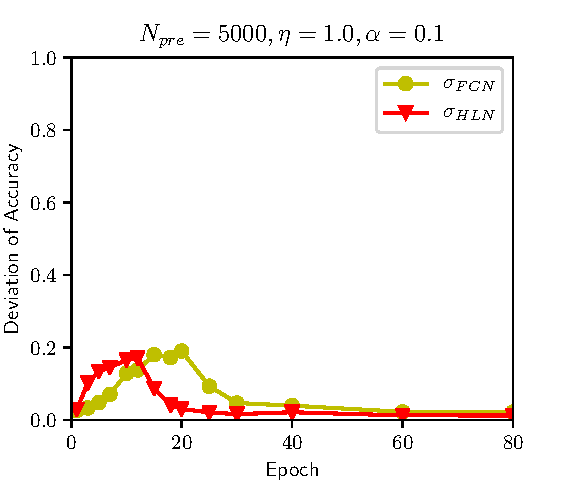
\includegraphics{fx1}\hspace*{5mm}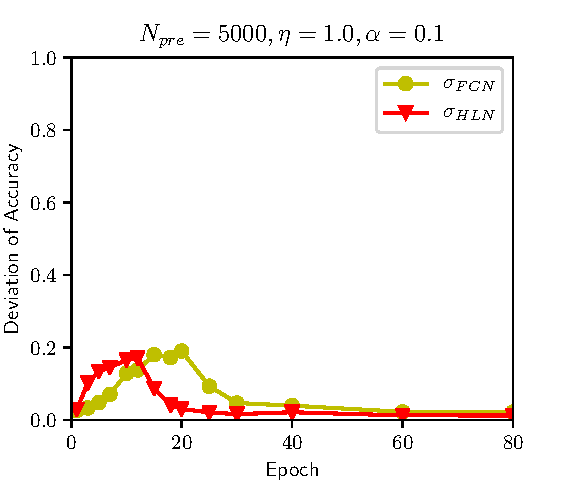
\includegraphics{fx1}}
\caption{(a) first picture; (b) second picture.}
\end{figure}


\begin{equation}
\begin{array}{rcl}
\displaystyle X_r &=& \displaystyle\dot{Q}^{"}_{rad}\left/\left(\dot{Q}^{"}_{rad} + \dot{Q}^{"}_{conv}\right)\right.\\[6pt]
\displaystyle \rho &=& \displaystyle\frac{\vec{E}}{J_c(T={\rm const.})\cdot\left(P\cdot\left(\displaystyle\frac{\vec{E}}{E_c}\right)^m+(1-P)\right)}
\end{array}
\end{equation}

They should also be separated from the surrounding text by one space.

\section{Conclusions}


\section*{Acknowledgements}

These and the Reference headings are in bold but have no numbers. Text below continues as normal.

%% References
%%
%% Following citation commands can be used in the body text:
%% Usage of \cite is as follows:
%%   \cite{key}         ==>>  [#]
%%   \cite[chap. 2]{key} ==>> [#, chap. 2]
%%


%% References with BibTeX database:

\bibliographystyle{elsarticle-num}
\bibliography{ref}

%% Authors are advised to use a BibTeX database file for their reference list.
%% The provided style file elsarticle-num.bst formats references in the required Procedia style

%% For references without a BibTeX database:

% \begin{thebibliography}{00}

%% \bibitem must have the following form:
%%   \bibitem{key}...
%%

% \bibitem{}

% \end{thebibliography}


%% The Appendices part is started with the command \appendix;
%% appendix sections are then done as normal sections
%% \appendix

%% \section{}
%% \label{}

\appendix
\section{An example appendix}
Authors including an appendix section should do so after References section. Multiple appendices should all have headings in the style used above. They will automatically be ordered A, B, C etc.

\subsection{Example of a sub-heading within an appendix}
There is also the option to include a subheading within the Appendix if you wish.

\end{document}

%%
%% End of file `procs-template.tex'.
